% =====================================================================
%  chunks/ch04b.tex —— 原书 p.153–164（PDF 160–171）
%  第 4 章 §1 基本概念、光滑纤维丛、联络、示性类（下）
% =====================================================================
% [原文 p.153]
由 (1.15)，这些关于 $\omega$ 与 $\Omega$ 在 $U\times\{1\}$ 上限制的局部公式，完全确定整个区域 $p^{-1}(U)\cong U\times G$ 上的 $\omega$ 与 $\Omega$。

当丛坐标改变，即微分同胚 $\phi_U$ 改变时，$\omega_{\phi_U}$ 与 $\Omega_{\phi_U}$ 的上述局部表达式如何变化？设 $\psi_U$ 是另一微分同胚 $p^{-1}(U)\to U\times G$，考虑微分同胚
\begin{equation}
\phi_U\psi_U^{-1}:U\times G\to U\times G,\qquad (x,g)\mapsto(x,\lambda(x)g), \tag{1.18}
\end{equation}
其中 $\lambda$ 确定相应的衔接函数，$\lambda(x)\in G$。特别地，截面 $U\times1$（$1\in G$ 是单位元）变到另一个截面：
\begin{equation}
\phi\psi^{-1}:(x,1)\mapsto(x,\lambda(x)),\qquad \lambda(x)\in G. \tag{1.19}
\end{equation}
（(1.19) 这种类型的变换在此语境中称为\emph{规范变换}。）在这一变换下，联络形式与曲率形式如下变换（假定 $G$ 与 $\cG$ 都由矩阵组成）：
\begin{equation}
\begin{aligned}
&\text{(i)}\qquad \omega_\phi\mapsto\omega_\psi,\qquad \omega_\phi=A_adx^a,\quad \omega_\psi=A'_adx^a,\\
&\qquad\qquad A_adx^a\mapsto A'_adx^a,\qquad A'_a=\lambda A_a\lambda^{-1}+(\partial_a\lambda(x))\lambda^{-1}(x);\\
&\text{(ii)}\qquad \Omega_\phi\mapsto\Omega_\psi,\\
&\qquad\qquad F_{ab}\mapsto\lambda(x)F_{ab}\lambda^{-1}(x)=F'_{ab}.
\end{aligned}
\tag{1.20}
\end{equation}

\begin{example*}{1}
设 $G$ 是 Abel Lie 群（例如 $G=S^1\cong SO_2\cong U_1$）。此时由 (1.16)，曲率形式本质上就是由联络形式 $\omega$ 在底空间上定义的闭 2-形式：
\[
p^*\Omega=d\omega.
\]
上同调类 $[\Omega]\in H^2(B;\R)$ 与联络的选取无关，并且是「整的」，即形式 $\Omega$ 在 2-闭链上的积分都是整数。
\end{example*}

\begin{example}{2}
设 $G=U_n$。此时任一曲率形式 $\Omega$ 的迹形式 $\Tr\Omega$（在局部坐标中即 $\Tr F_{ab}dx^a\wedge dx^b$）又是底空间上的闭 2-形式，其上同调类
\[
[\Tr\Omega]=c_1\in H^2(B;\R)
\]
与联络的选取无关，且为整值。这个上同调类称为 $B$ 的\emph{第一 Chern 类}。由矩阵 $(F_{ab})$ 取幂所得的 $\Tr(\Omega^m)$ 代表整上同调类 $\tilde c_m\in H^{2m}(B;\R)$（或复系数），它们也称为 $B$ 的 \emph{Chern 类}。不过对整 Chern 类（其精确定义见下文），有更合适的基 $c_1,c_2,\ldots$，使类 $\tilde c_i$ 可用整数多项式表示（反之则不行）：
% [原文 p.154]
\[
\tilde c_i=P_i(c_1,\ldots,c_i).
\]
多项式 $P_i(c_1,\ldots,c_i)$ 实际上就是 Newton 多项式，它把对称多项式 $\sum_{k=1}^n u_k^i$ 用初等对称多项式
\[
c_j=\sum_{i_1<\cdots<i_j}u_{i_1}\cdots u_{i_j};\qquad \tilde c_1=c_1,\quad \tilde c_2=c_1^2-2c_2,\quad\ldots
\]
表示出来。把类 $\tilde c_i$、$c_i$ 表示为对称多项式，这一做法具有拓扑意义，并且极为有用（见下文）。
\end{example}

% [Tutor Note: 例 1、例 2 的关键点在于：由曲率形式构造的上同调类与联络的选取无关，故它实际上是丛（或底空间）的不变量；这正是「示性类可用曲率表示」的第一批例子。]
\begin{example}{3}
设 $G=SO_n$。此时（任一联络的）曲率形式 $\Omega$ 给出 $B$ 的 \emph{Pontryagin 类} $\tilde p_i=[\Tr\Omega^{2i}]\in H^{4i}(B;\R)$，它们也是整值的。与 Chern 类的情形一样，下文我们将为 Pontryagin 类选取另一组基 $p_i$（在 $\Z$ 上「不可分」），而 $\tilde p_i$ 同样可用 Newton 多项式表达。
\end{example}

主 $G$-丛全空间上决定该丛之联络的「水平 $n$ 维切子空间场」（按定义），在任一相伴丛 $(E',B,F,G,p')$ 的全空间 $E'$ 上诱导出同样与纤维横截的这类子空间场。借助这一水平切子空间场，底 $B$ 中每条光滑或分段光滑道路 $\gamma(t)$（$a\le t\le b$）都被 $E'$ 中唯一一条水平道路 $\tilde\gamma(t)$ 覆叠，即 $p'\tilde\gamma(t)=\gamma(t)$，只要给定初始点 $\tilde\gamma(a)$（见图 4.3）。

\begin{center}
\begin{minipage}{\textwidth}\centering
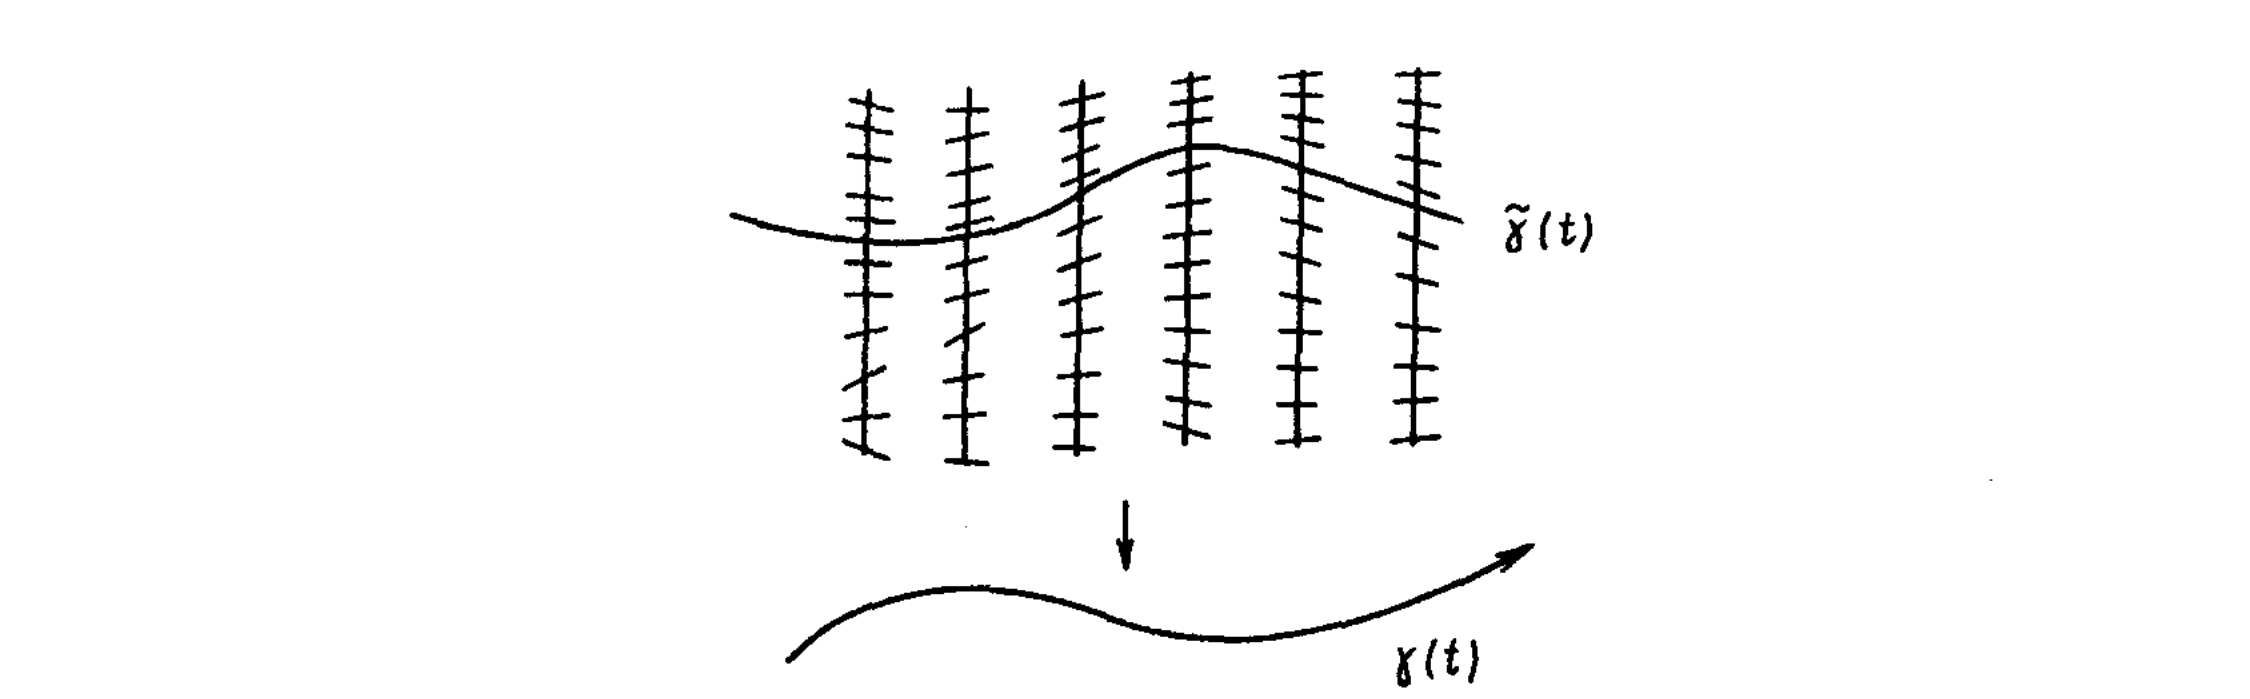
\includegraphics[width=0.70\textwidth]{figures/fig4_3.png}\par
\figtitle{4.3}{图中：底空间中的道路 $\gamma(t)$ 与其在全空间中的水平提升 $\tilde\gamma(t)$。}
\end{minipage}
\end{center}

点 $\tilde\gamma(t)$ 在 $\gamma(t)$ 之上的这种覆叠运动称为\emph{平行移动}。「水平子空间场」这一构造正是第 2 章 §3 引入的「同伦联络」的光滑版本，它带有相应的「覆叠同伦性质」，以及由此导出的同伦推论。

% [Tutor Note: 平行移动把「联络」变成可计算的东西：沿闭路平行移动得到的纤维自同构即和乐（holonomy）。它与第 2 章的同伦提升性质是同一件事在光滑范畴中的实现。]
% [原文 p.155]
主 $G$-丛上的联络决定沿底 $B$ 的任一切向量方向、在任意相伴 $G$-丛的截面上作\emph{协变微分}的运算。如上所述，用底 $B$ 的适当区域 $U$ 上的局部坐标，联络 1-形式为
\[
\omega_{\phi_U}=A_a(x)dx^a.
\]
由于 $A_a$ 是矩阵值函数，可写 $A_a=(A_a)_i^j=(A_{aj}^i)$，$i,j=1,\ldots,q$。相伴 $G$-丛的一个截面局部地可表示为取值于 $\R^n$ 的向量值函数 $(\eta^i(x))$。于是协变导数就是如下定义的算子 $D_a$：
\begin{equation}
D_a=\partial_a+A_a,\qquad D_a\eta^i(x)=\partial_a\eta^i+A_{aj}^i\eta^j. \tag{1.21}
\end{equation}
换位子 $[D_a,D_b]$ 给出曲率分量 (1.17)：
\begin{equation}
[D_a,D_b]=\partial_aA_b-\partial_bA_a+[A_a,A_b]=F_{ab}. \tag{1.22}
\end{equation}

对切丛 $\tau(M^n)$，上述讨论给出 Riemann 几何的经典概念。纤维丛上联络这一思想，最初似由 Weyl 在 1930 年代就特殊情形引入，而由 Cartan 以一般形式引入。物理学家稍晚一些（Yang 与 Mills，1950 年代中期）独立地达到这一概念——至少独立于 Cartan。在物理术语中，联络称为「规范场」；它们在基本粒子物理中具有根本重要性。这种场最简单的例子（属于 Weyl）是 $G=U_1\cong SO_2\cong S^1$ 的 $G$-丛上的联络，其物理解释是电磁场，场强即曲率张量 $F_{ab}$。如上所述（见 (1.20)），规范变换正是联络局部公式的那些变换，它们由从恒同截面变到另一截面而产生：$(x,1)\mapsto(x,\lambda(x))$。在 Einstein 的广义相对论中，人们考虑切丛上由引力场产生的联络。

回到我们论述的主线，现在引入光滑 $G$-丛的「示性类」概念。

\begin{definition*}{1.1}
关于 $G$-丛范畴 $(E,B,F,G,p)$ 的\emph{示性类} $\theta$，是给每个 $G$-丛对应一个元素 $\theta\in H^*(B)$（某系数环上）的函数，使得在丛映射 $\Phi:E\to E'$、$\phi:B\to B'$ 下示性类表现自然（更确切地说，作为反变函子）：
\[
\phi^*(\theta')=\theta,\qquad \phi:B\to B'.
\]
\end{definition*}

容易看出：$G$-丛的示性类与万有 $G$-丛的底 $BG$ 的上同调环的元素一一对应。因为前面已指出，底为 $B$ 的每个 $G$-丛都可由映射 $\phi:B\to BG$（同伦意义下唯一）诱导出；于是若给定了 $\theta'\in H^*(BG)$，便可把 $\phi$ 诱导的 $B$ 上 $G$-丛的示性类取为 $\theta'$ 的拉回：$\theta=\phi^*(\theta')$。

% [原文 p.156]
对紧 Abel 群 $G$，空间 $BG$ 是已知的：
\[
\begin{aligned}
&G=S^1, && BG=\CP^\infty,\\
&G=T^n, && BG=\CP_1^\infty\times\cdots\times\CP_n^\infty;\\
&G=(\Z/2)^n, && BG=\RP_1^\infty\times\cdots\times\RP_n^\infty;\\
&G=\Z/m, && BG=\lim_{n\to\infty}S^{2n-1}/\Z/m=S^\infty/\Z/m,
\end{aligned}
\]
（最后一式中 $S^\infty/\Z/m$ 是无穷维透镜空间。）这些 $BG$ 的上同调环也是已知的；其中特别重要的有：
\begin{equation}
\begin{aligned}
&H^*(\CP_1^\infty\times\cdots\times\CP_n^\infty;\Z)\cong\Z[u_1,\ldots,u_n],\\
&\qquad(\text{$\Z$ 上关于 }u_j\in H^2(\CP_j^\infty;\Z)\text{ 的多项式环});\\
&H^*(\RP_1^\infty\times\cdots\times\RP_n^\infty;\Z/2)\cong\Z/2[v_1,\ldots,v_n],\qquad v_j\in H^1(\RP_j^\infty;\Z/2);\\
&H^*(B\Z/p;\Z/p)=\Lambda_p(v)\otimes\Z/p[u],\\
&\qquad v\in H^1(B\Z/p;\Z/p),\qquad u=\beta v\in H^2(B\Z/p;\Z/p),
\end{aligned}\tag{1.23}
\end{equation}
其中 $\beta$ 是 Bockstein 同态（见第 3 章 §5），$\Lambda_p(v)$ 是由 $v$ 生成的 $\Z/p$ 上的外代数（$v^2=0$），并且张量积上附加了斜交换性。

% [Tutor Note: (1.23) 给出的是分类空间的模 $p$ 上同调环：$\Z/p$ 系数时 Bockstein 同态 $\beta$ 把 $1$ 维类 $v$ 送到 $2$ 维类 $u=\beta v$，这是证明「分类空间的上同调环完全决定了示性类」的关键计算工具。]

对 $G=O_n$、$SO_n$、$U_n$、$SU_n$，上同调环 $H^*(BG)$（系数取 $\Z$、$\Z/2$ 或 $\R$）的最重要事实如下。

在群 $U_n$ 中有子群 $T^n$，即由对角矩阵 $g$ 组成的\emph{极大环面}，以及由正规化 $T^n$ 的置换矩阵 $g$（$gT^ng^{-1}=T^n$）组成的 \emph{Weyl 群} $S_n$。上同调环 $H^*(BU_n)$ 到 $H^*(BT^n)$ 的限制有零核，即由包含 $i:BT^n\to BU_n$ 诱导的同态
\[
i^*:H^*(BU_n;\Z)\to H^*(BT^n;\Z)\cong\Z[u_1,\ldots,u_n]
\]
是单射，且在 Weyl 群作用下不变。由此可知，空间 $BU_n$ 的上同调环经由 $i^*$ 由 $BT^n$ 的上同调环给出，而 $i^*$ 的像由 $u_1,\ldots,u_n$ 的全部对称多项式组成，从而给出环 $H^*(BU_n;\Z)$ 的完整描述。Chern 类 $c_i\in H^{2i}(BU_n;\Z)$ 定义为被 $i^*$ 映到「Wu 变量」（即元素 $u_j\in H^2(\CP_j^\infty;\Z)$）中第 $i$ 个初等对称多项式的元素：

% [原文 p.157]
\begin{equation}
c_i\mapsto\sum_{j_1<\cdots<j_i}u_{j_1}\cdots u_{j_i},\qquad \tilde c_i\mapsto\sum_{j=1}^n u_j^i. \tag{1.24}
\end{equation}
于是元素 $c_i$ 构成 $H^*(BU_n;\Z)$ 的一组基。（元素 $\tilde c_i$ 早先是用曲率形式定义的。）

对群 $SO_{2n}$、$SO_{2n+1}$，极大环面 $T^n$ 与 $U_n$ 的情形相同，但 Weyl 群更大。限制同态
\[
H^*(BSO_k;\Z)\to H^*(BT^n;\Z),\qquad k=2n,\ 2n+1,
\]
（类似于上面的 $i^*$）的核只含 2-挠元素。$SO_{2n}$ 的 Weyl 群（通过它在 $H^*(BT^n;\Z)$ 上的作用来描述）由 $u_1,\ldots,u_n$ 的全部置换所成的对称群 $S_n$，以及由
\begin{equation}
\sigma_{ij}:u_i\mapsto -u_i,\quad u_j\mapsto -u_j,\quad u_k\mapsto u_k,\quad k\ne i,j \tag{1.25}
\end{equation}
定义的变换 $\sigma_{ij}$ 一起生成。对 $SO_{2n+1}$，则代替这些变换，需要以
\begin{equation}
\sigma_i:u_i\mapsto -u_i,\qquad u_j\mapsto u_j,\qquad j\ne i \tag{1.26}
\end{equation}
给出的变换作为生成元。于是 $SO_{2n+1}$ 的不变多项式集合比 $SO_{2n}$ 的小。

同态 $H^*(BSO_{2n};\Z)\to H^*(BT^n;\Z)$ 在 Weyl 群作用下的不变性表明：其像由平方 $u_j^2$ 的初等对称多项式的线性组合组成，这些多项式代表 \emph{Pontryagin 类} $p_i$。再添上多项式 $\chi_{2n}=u_1\cdots u_n$，它代表\emph{Euler 示性类}。另一方面，限制同态 $H^*(BSO_{2n+1};\Z)\to H^*(BT^n;\Z)$ 的像仅由 Pontryagin 类的像张成。概括起来（对 $SO_{2n}$、$SO_{2n+1}$ 皆然）：
\begin{equation}
\begin{aligned}
&p_i\mapsto\sum_{j_1<\cdots<j_i}u_{j_1}^2\cdots u_{j_i}^2\in H^{4i}(BT^n;\Z),\\
&\chi_{2n}\mapsto u_1\cdots u_n\in H^{2n}(BT^n;\Z),\\
&p_i\in H^{4i}(BSO_k;\Z),\quad k\ge2n,\qquad \chi_{2n}\in H^{2n}(BSO_{2n};\Z).
\end{aligned}\tag{1.27}
\end{equation}

在实数域 $\R$（或 $\Q$）上，对一切紧 Lie 群 $G$（极大环面为 $T^n$）情形相同：限制同态 $H^*(BG;\R)\to H^*(BT^n;\R)$ 的核平凡，像由 $u_1,\ldots,u_n$ 在 Weyl 群诱导作用下的全部不变多项式组成。

为描述 $BG$（$G=O_n,SO_n$）的模 2 上同调，人们使用环面的显然离散类比，即对角矩阵子群 $(\Z/2)^n\subset O_n$。这里限制同态
\[
H^*(BO_n;\Z/2)\to H^*(B(\Z/2)^n;\Z/2)\cong\Z/2[v_1,\ldots,v_n],
\]
\[
v_j\in H^1(\RP_j^\infty;\Z/2),\qquad B\Z/2=\RP^\infty,
\]
的核平凡，像由 $v_1,\ldots,v_n$ 的对称多项式组成。
% [原文 p.158]
$H^*(BO_n;\Z/2)$ 中在此同态下映到 $v_1,\ldots,v_n$ 的第 $j$ 个初等对称多项式的元素，称为 \emph{Stiefel--Whitney 示性类} $w_j$：
\begin{equation}
w_j\mapsto\sum_{i_1<\cdots<i_j}v_{i_1}\cdots v_{i_j}\in H^j(B(\Z/2)^n;\Z/2). \tag{1.28}
\end{equation}
自然同态 $H^*(BO_n;\Z/2)\to H^*(BSO_n;\Z/2)$ 是满的（即满同态），其核是由 $w_1$ 生成的主理想，即 $w_1$ 的倍数组成的集合。

注意：Chern 类 $c_i$ 模 2 约化给出 Stiefel--Whitney 类 $w_{2i}$，而 $\chi_{2n}$ 模 2 约化给出 $w_{2n}$：
\[
w_{2i}=c_i\ (\mathrm{mod}\ 2),\qquad w_{2n}=\chi_{2n}\ (\mathrm{mod}\ 2).
\]
还注意：
\[
p_i(\eta)\ (\mathrm{mod}\ 2)=w_{4i}(c\eta)=\sum_{2j+2k=2i}w_{2j}(\eta)w_{2k}(\eta),
\]
（其中 $c$ 表示「复化」），而对 $U_n$-丛有 $\chi_{2n}=c_n$。

\emph{流形的示性类}定义为该流形切丛的示性类。

以上就是关于示性类的基本事实。下面描述它们的一些进一步性质。

首先注意：条件 $w_1(\eta^n)=0$ 是 $G$-丛 $\eta^n$ 可定向，即丛的结构群 $G$ 可归约到 $SO_n$ 的充要条件。

回忆：对以 $B$ 为底的任意实（或复）向量丛 $\eta^n$，可伴随一个（底为 $B$ 的）纤维化，其纤维为
\[
F=V^\R_{n,n-k}\qquad(\text{或}\ F=V^\C_{n,n-k}),
\]
即相应的 Stiefel 流形。Stiefel--Whitney 类（复情形为 Chern 类）正是这一纤维丛截面存在性的「第一障碍」（见第 3 章 §6）：
\[
V^\R_{n,n-k}(\eta^n)\xrightarrow{V^\R_{n,n-k}}B\qquad(\text{复情形为}\ V^\C_{n,n-k}(\eta^n)\xrightarrow{V^\C_{n,n-k}}B),
\]
其中
\[
\pi_j(F)=0,\quad j<k-1,\qquad \pi_{k-1}(F)\otimes\Z/2\cong\Z/2,\qquad F=V^\R_{n,n-k},
\]
或
\[
\pi_j(F)=0,\quad j<2k-1,\qquad \pi_{2k-1}(F)\cong\Z,\qquad F=V^\C_{n,n-k}.
\]

% [原文 p.159]
在第一种情形（$F=V^\R_{n,n-k}$）中，基本群 $\pi_1(B)$ 平凡地作用于群 $\pi_{k-1}(F)\otimes\Z/2$；在第二种情形（$F=V^\C_{n,n-k}$）中则平凡地作用于 $\pi_{2k-1}(F)$，其中原向量丛 $\eta^n$ 的结构群分别是 $O_n$、$U_n$（甚至可以是 $GL_n(\R)$、$GL_n(\C)$）。

示性闭链 $w_i$、$c_i$ 的 Poincaré 对偶 $Dw_i$、$Dc_i$（作为相应同调群中的闭链）的构造更为直接。对类 $w_i$，取任意以光滑闭流形 $B$ 为底、纤维为 $\R^n$ 的 $O_n$-丛 $\eta^n$，并考虑 $B$ 上处于一般位置的 $k$ 元向量组场 $v_1(x),\ldots,v_k(x)$（$x\in B$）；于是使向量 $v_1(x),\ldots,v_k(x)$ 线性相关的全部点 $x\in B$ 构成维数为 $n-k+1$ 的（模 2）闭链，它代表元素 $Dw_i$。换言之，若考虑 $B$ 上相伴纤维丛 $V^\R_{n,n-k}(\eta^n)$ 的一个处于一般位置的截面，则该截面的全部「零点」构成代表 $Dw_i$ 的闭链。对定向（或 $SO_n$-）丛 $\eta^n$，若 $n=2m$、$k=1$，上述场就是向量场，其零点构成维数为 $n$ 的整闭链，代表元素 $D\chi_{2m}$。Chern 类的对偶可类似地得到。

对 $G$-丛，子群 $G_1\subset G$ 常被用作结构群；在可能时把结构群取为子群的运算，称为结构群 $G$ 的\emph{归约}。在一类等价 $C^\infty$-丛中，结构 Lie 群 $G$ 总可归约到极大紧子群。（然而在一类等价复解析 $G$-丛中，这并不总是可能。）

任一复向量丛 $\eta$ 都可通过「忘掉」复结构而视为实的：$\eta\mapsto r\eta$；这一运算对应嵌入 $U_n\xrightarrow{r}SO_{2n}$（或 $GL_n(\C)\xrightarrow{r}GL_{2n}(\R)$）。另一方面，对任意实向量丛 $\eta$ 可施行\emph{复化}运算 $\eta\mapsto c\eta$，使用嵌入 $GL_n(\R)\xrightarrow{c}GL_n(\C)$。给定一个群到另一个群的表示（即同态）$\rho:G_1\to G_2$，由任意 $G_1$-丛 $\eta$ 按显然方式得到 $G_2$-丛 $\rho\eta$。下面列出这些以及向量丛的其他运算（其中一些前面已提到）：

1. 直和 $\eta_1\oplus\eta_2$。

2. 张量积 $\eta_1\otimes\eta_2$（在 $\R$ 或 $\C$ 上）。

3. 外幂 $\Lambda^j\eta$（当 $j=n=\dim\eta$ 时与丛的\emph{行列式}一致：$\det\eta=\Lambda^n\eta$）。

4. 对称幂 $S^j\eta$（张量幂 $\otimes^j\eta$ 的对称部分）。于是
\begin{equation}
\Lambda^2\eta\oplus S^2\eta=\eta\otimes\eta. \tag{1.29}
\end{equation}

5. 对偶丛 $\eta^*$；复共轭丛 $\bar\eta$（当 $\eta$ 是复丛时）；上面提到的运算 $r$ 与复化 $c$，它们满足
\begin{equation}
rc(\eta)\cong\eta\oplus\eta^*,\qquad c\bar\eta\cong c\eta,\qquad cr(\eta)\cong\eta\oplus\bar\eta. \tag{1.30}
\end{equation}

% [原文 p.160]
由定义可知，向量丛 $\eta$ 的 Pontryagin 类与复化丛 $c\eta$ 的 Chern 类（相差符号）一致：
\begin{equation}
(-1)^ip_i(\eta)=c_{2i}(c\eta),\qquad 2c_{2i+1}(c\eta)=0. \tag{1.31}
\end{equation}
对向量丛的直和，下列公式成立：
\begin{equation}
\begin{aligned}
\text{(i)}&\qquad w_i(\eta_1\oplus\eta_2)=\sum_{j+k=i}w_j(\eta_1)w_k(\eta_2),\qquad w_0=1;\\
\text{(ii)}&\qquad c_i(\eta_1\oplus\eta_2)=\sum_{j+k=i}c_j(\eta_1)c_k(\eta_2),\qquad c_0=1;\\
\text{(iii)}&\qquad p_i(\eta_1\oplus\eta_2)=\sum_{j+k=i}p_j(\eta_1)p_k(\eta_2),\qquad \text{模 2-挠};\\
\text{(iv)}&\qquad \chi_{2n}(\eta_1\oplus\eta_2)=\chi_{2k}(\eta_1)\chi_{2m}(\eta_2),\qquad k+m=n,
\end{aligned}\tag{1.32}
\end{equation}
其中在 (iv) 中假定 $\dim\eta_1=2k$、$\dim\eta_2=2m$。

由这些公式可知：除 $\chi_{2n}$ 外，这些类都是\emph{稳定的}，即若 $\varepsilon_\R^N$（或 $\varepsilon_\C^N$）是纤维为 $\R^N$（或 $\C^N$）的平凡丛，则
\[
w_i(\eta\oplus\varepsilon_\R^N)=w_i(\eta),\qquad c_i(\eta\oplus\varepsilon_\C^N)=c_i(\eta),\qquad p_i(\eta\oplus\varepsilon_\R^N)=p_i(\eta).
\]

% [Tutor Note: (1.31)(1.32) 的要点是把示性类解释为形式变量 $u_1,\ldots,u_n$ 上的对称多项式：对直和 $\eta=\eta_1\oplus\eta_2$ 只要把两组形式变量并起来，(1.32) 就成了初等对称多项式的乘法；使 $\eta$ 形式上分裂成线丛之和的这种想法称为分裂原理。]

示性类在 $B$ 上向量丛的张量积运算（以及外幂、对称幂运算）下的行为要复杂一些。这种行为可以在有理（或实）上同调中借助极大环面上同调环 $H^*(T^n;\Q)$ 的「Wu 生成元」 $u_1,\ldots,u_n$ 来描述。对 $U_n$-丛 $\eta$，\emph{Chern 特征标} $\ch(\eta)$ 定义为形式级数
\begin{equation}
\begin{aligned}
&\ch(\eta)=\sum_{j=1}^n\exp(u_j)=\sum_{j=1}^n\sum_{m\ge0}\frac{u_j^m}{m!}=\sum_{m\ge0}\frac1{m!}\tilde c_m=\sum_{m\ge0}\ch_m(\eta),\\
&\ch_m(\eta)=\frac1{m!}\tilde c_m=P_m(c_1,\ldots,c_m),
\end{aligned}\tag{1.33}
\end{equation}
而对 $SO_n$-丛 $\eta$，
\[
\ch(\eta)=\ch(c\eta),
\]
其中 $\ch(c\eta)$ 由 (1.33) 给出。这里我们把 $u_1,\ldots,u_n$ 的初等对称多项式与 Chern 类 $c_i$ 等同（并把 $u_1^2,\ldots,u_n^2$ 的初等对称多项式与 Pontryagin 类 $p_i$ 等同）。于是有简单公式
\begin{equation}
\ch(\eta_1\otimes\eta_2)=\ch\eta_1\ch\eta_2. \tag{1.34}
\end{equation}

下文我们将常常省略张量积的符号 $\otimes$，因为对丛没有别的乘积。为暂时回到
$B$ 上向量丛之和 $\eta_1\oplus\eta_2$ 的示性类，我们考虑形式级数（对每个向量丛 $\eta$ 定义）：
% [原文 p.161]
\[
1\oplus\eta\oplus\Lambda^2\eta\oplus\Lambda^3\eta\oplus\cdots=\Lambda(\eta),
\]
\[
1\oplus\eta\oplus S^2\eta\oplus S^3\eta\oplus\cdots=S(\eta),
\]
容易看出它们满足
\begin{equation}
\begin{aligned}
&\Lambda(\eta_1\oplus\eta_2)=\Lambda(\eta_1)\Lambda(\eta_2),\\
&S(\eta_1\oplus\eta_2)=S(\eta_1)S(\eta_2).
\end{aligned}\tag{1.35}
\end{equation}
类似地，若（形式地）记
\[
w=1+w_1+w_2+\ldots,\qquad c=1+c_1+c_2+\ldots,\qquad p=1+p_1+p_2+\ldots,
\]
则公式 (1.32) 具有简单形式：
\[
\begin{aligned}
\text{(i)}&\qquad w(\eta_1\oplus\eta_2)=w(\eta_1)w(\eta_2),\\
\text{(ii)}&\qquad c(\eta_1\oplus\eta_2)=c(\eta_1)c(\eta_2),\\
\text{(iii)}&\qquad p(\eta_1\oplus\eta_2)=p(\eta_1)p(\eta_2)\quad(\text{模 2-挠}).
\end{aligned}
\]

符号生成元 $u_1,\ldots,u_n$（代表 $H^*(BT^n;\R)$ 的适当元素）也便于用来定义示性类中的加性与乘性表达式 $f(\eta)$（如 $w(\eta)$、$c(\eta)$、$p(\eta)$）。结果表明，一切这样的加性表达式（即满足 $f(\eta_1\oplus\eta_2)=f(\eta_1)+f(\eta_2)$ 者）都可以从单变量 $u$ 的相应表达式得到。后者的形式如下：成幂级数（分别对复丛与实丛）：
\[
\begin{aligned}
\text{(i)}&\qquad f(u)=\sum_{m\ge0}a_mu^m,\qquad f(\eta)=f(c_1,\ldots,c_k,\ldots)=\sum_{j=1}^nf(u_j);\\
\text{(ii)}&\qquad f(u^2)=\sum_{m\ge0}b_mu^{2m},\qquad f(\eta)=f(p_1,\ldots,p_k,\ldots)=\sum_{j=1}^nf(u_j^2).
\end{aligned}
\]
于是所有加性表达式 $f(u)$ 都具有形式（同样分别对复丛与实丛）：
\begin{equation}
\begin{aligned}
\text{(i)}&\qquad f(\eta)=f(c_1,\ldots,c_k,\ldots)=\sum_{m\ge0}m!a_m\tilde c_m=\sum_{m\ge0}m!a_m\ch_m(\eta);\\
\text{(ii)}&\qquad f(\eta)=f(p_1,\ldots,p_k,\ldots)=\sum_{m\ge0}m!b_m\tilde c_{2m}=\sum_{m\ge0}m!b_m\ch_{2m}(\eta).
\end{aligned}\tag{1.36}
\end{equation}

% [原文 p.162]
类似地，一切乘性特征标 $f(\eta)$（即满足 $f(\eta_1\otimes\eta_2)=f(\eta_1)\cdot f(\eta_2)$ 者）都由单变量的幂级数确定，其形式如下：
\[
\begin{aligned}
\text{(i)}&\qquad f(u)=\sum_{m\ge0}a_mu^m,\qquad f(\eta)=f(c_1,\ldots,c_k,\ldots)=\prod_{j=1}^nf(u_j);\\
\text{(ii)}&\qquad f(u^2)=\sum_{m\ge0}b_mu^{2m},\qquad f(\eta)=f(p_1,\ldots,p_k,\ldots)=\prod_{j=1}^nf(u_j^2).
\end{aligned}
\]
在闭流形（实或复）上，乘性特征标 $f$ 的形式由下列要求确定：
\[
f(M_1^n\times M_2^m)=f(M_1^n)\cdot f(M_2^m),
\]
由此得到：
\[
\text{(i)}\qquad f(M^{2n})=\langle f(c_1,\ldots,c_n),[M^{2n}]\rangle\quad(\text{复情形});
\]
\[
\text{(ii)}\qquad f(M^{4n})=\langle f(p_1,\ldots,p_n),[M^{4n}]\rangle\quad(\text{实可定向情形}).
\]
特别地，在上述情形 (i) 中，对 Euler 示性数 $\chi[M^{2n}]$ 有
\[
f(u)=1+u,\qquad f(c_1,\ldots,c_k,\ldots)=1+c_1+c_2+\ldots.
\]
下文我们还会遇到其他重要情形。

\begin{example*}{1}
对 $n$ 维实射影空间 $\RP^n$ 的切丛 $\tau=\tau(\RP^n)$，有简单的丛同构
\[
\tau(\RP^n)\oplus\varepsilon_\R\cong\underbrace{\eta\oplus\cdots\oplus\eta}_{n+1\ \text{个}},
\]
其中 $\varepsilon_\R$ 表示 $\RP^n$ 上纤维为 $\R^1$ 的平凡丛，而 $\eta$ 是 $\RP^n$ 上结构群为 $O_1\cong\Z/2$ 的唯一非平凡线丛。在 $\RP^1$ 上，$\eta$ 的全空间就是通常的 Möbius 带（见图 4.4）——只是纤维取为开区间。$\eta$ 的 Stiefel--Whitney 类如下：
\[
0\ne w_1(\eta)=v\in H^1(\RP^n;\Z/2),\qquad w_i(\eta)=0,\quad i>1.
\]
闭链 $Dv\in H_{n-1}(\RP^n;\Z/2)$ 由超曲面 $\RP^{n-1}\subset\RP^n$ 代表；见图 4.5。用向量丛直和的公式，由此得到
\[
w(\tau)=1+w_1(\tau)+\ldots+w_n(\tau)=(1+v)^{n+1}\in H^*(\RP^n;\Z/2).
\]
\end{example*}

% [原文 p.163]
\begin{center}
\begin{minipage}{\textwidth}\centering
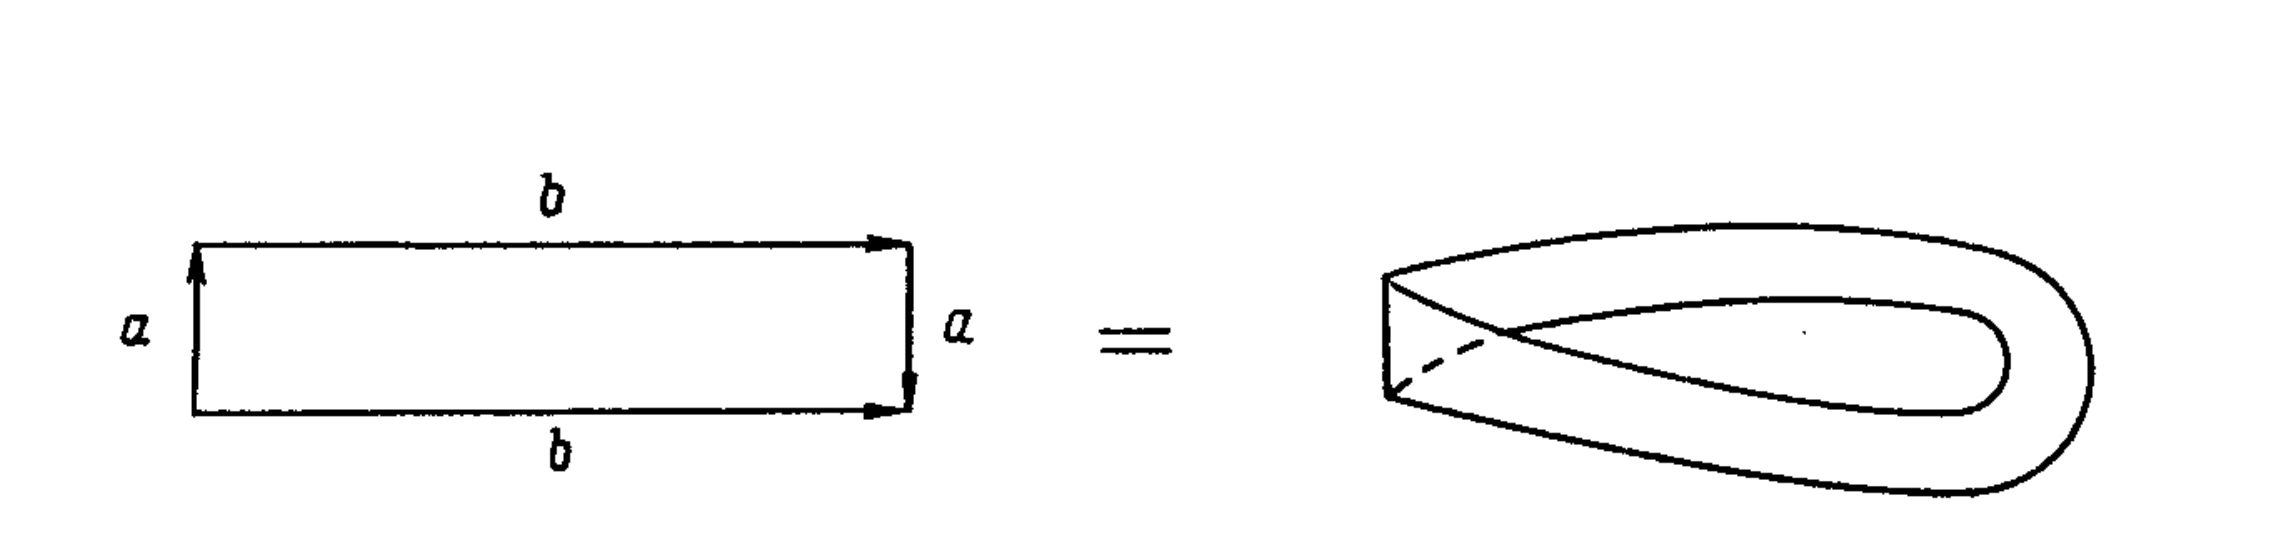
\includegraphics[width=0.80\textwidth]{figures/fig4_4.png}\par
\figtitle{4.4}{Möbius 带：最简单的非平凡丛，底为 $S^1$，纤维为区间。}
\end{minipage}
\end{center}

\begin{center}
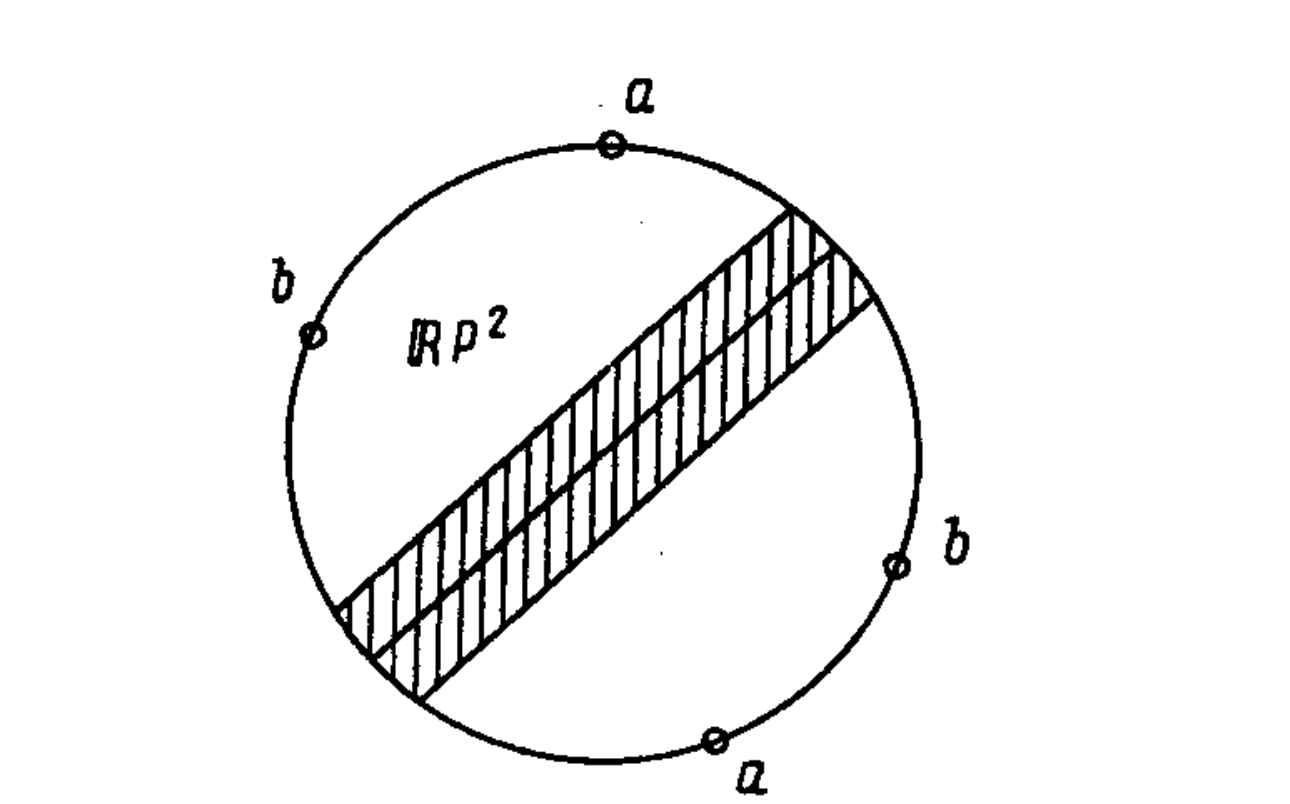
\includegraphics[width=0.46\textwidth]{figures/fig4_5.png}
\end{center}
\figtitle{4.5}{图中：射影平面 $\RP^2$ 及其中的射影直线 $\RP^1$（阴影带）。}

% [Tutor Note: 例 1 用 Möbius 带演示了「示性类是障碍」这一思想：$\eta$ 非平凡，故 $w_1(\eta)\ne0$；而 $w(\tau)=(1+v)^{n+1}$ 说明实射影空间的 Stiefel--Whitney 类完全由其上同调环的生成元决定。]
\begin{example*}{2}
切丛 $\tau=\tau(\CP^n)$ 是复 $GL_n(\C)$-丛。与前例类似的理由给出
\[
\tau(\CP^n)\oplus\varepsilon_\C\cong\underbrace{\eta\oplus\cdots\oplus\eta}_{n+1\ \text{个}},
\]
\[
c_1=u\in H^2(\CP^n;\Z),
\]
\[
c(\tau)=1+c_1(\tau)+\ldots+c_n(\tau)=(1+u)^{n+1}\in H^*(\CP^n;\Z),
\]
其中 $u$ 是 $H^2(\CP^n;\Z)\cong\Z$ 的生成元。Poincaré 对偶闭链 $Du\in H_{2n-2}(\CP^n;\Z)$ 由闭链 $\CP^{n-1}\subset\CP^n$ 代表。
\end{example*}

\begin{example*}{3}
设 $M^n$ 是光滑流形 $N^k$ 的光滑子流形（$n<k$）。此时除切丛 $\tau=\tau(M^n)$ 外，我们还有 $M^n$ 在 $N^k$ 中关于 $N^k$ 上某个 Riemann 度量的\emph{法丛} $\nu=\nu(M^n)$（事实上度量在这里并不重要）。有简单公式
\[
i^*\tau(N^k)=\tau(M^n)\oplus\nu(M^n)
\]
（其中 $i^*$ 由包含 $i:M^n\to N^k$ 诱导），于是
\[
i^*w(N^k)=w(\tau)w(\nu),
\]
\[
i^*p(N^k)=p(\tau)p(\nu)\qquad(\text{模 2-挠}),
\]
\[
i^*c(N^k)=c(\tau)c(\nu),
\]
最后一式对复 $U_n$-流形 $M^n\subset N^k$ 成立。
% [原文 p.164]
在 $N^k=\R^k$ 的情形，切丛 $\tau(\R^k)$ 平凡，故
\[
i^*w(\R^k)=1,\qquad i^*p(\R^k)=1.
\]
因此 $w(\tau)w(\nu)=1$ 且 $p(\tau)p(\nu)=1$（模 2-挠），从而得到（见 (1.32)）用彼此表示 $M^n$ 的切丛与法丛相应示性类的公式。
\end{example*}

\begin{example*}{4}
对偶数维可定向流形 $M^{2n}$ 的切丛 $\tau$，Euler 示性类满足
\[
\langle\chi_{2n}(\tau),[M^{2n}]\rangle=\chi(M^{2n}),
\]
即在基本同调类 $[M^{2n}]$ 上取值时给出 Euler--Poincaré 示性数。（对 $U$-流形，把类 $\chi_{2n}$ 换成 Chern 类 $c_n$。）
\end{example*}

\begin{example*}{5}
对 Lie 群 $G$，切丛平凡，因而一切示性类为零。Lie 群是可平行化流形，即容许处处非退化的 $n$-标架场（$n=\dim G$）（由单位元处切空间的任一基经左（或右）平移得到）。
\end{example*}

\begin{example}{6}
设 $\R^N$ 的子流形 $M^n$ 由方程组 $f_1=0,\ldots,f_{N-n}=0$ 定义，其中 $f_i$ 的梯度（$i=1,\ldots,N-n$）在公共零点流形上处处线性无关：
\[
M^n=\{x\in\R^N\mid f_1(x)=0,\ldots,f_{N-n}(x)=0\}.
\]
此时法丛 $\nu(M^n)$（纤维为 $\R^{N-n}$）平凡；由公式 (1.32)，流形 $M^n$ 的一切稳定示性类 $w_i$、$p_k$ 都为零。只有 Euler 类 $\chi_{2k}$ 可能非零，且必须 $n=2k$。（例如 $\chi(S^{2k})=2$。）这里切丛 $\tau(M^n)$ 稳定平凡，即 $\tau\oplus\varepsilon_\R^{N-n}=\varepsilon_\R^N$。
\end{example}

上文多处提到\emph{复流形}的概念：它是偶数维实光滑流形，其坐标卡 $V_\alpha$ 用复坐标 $z_\alpha^1,\ldots,z_\alpha^n$ 作坐标，而在重叠区域 $V_\alpha\cap V_\beta$ 上衔接函数是复解析的。这里 $n$ 是复流形 $M^n$ 的\emph{复维数}；作为实流形，它的维数是 $2n$。

% CHUNK ch04b DONE
